\chapter[Prototype Codex]{L'évolution architecturale de la bibliothèque numérique}
\lettrine{L}e passage de la définition des besoins des personnels de la bibliothèque Cujas ainsi que des usagers à l'implémentation d'une infrastructure informatique opérationnelle marque un tournant technique dans la refonte de CujasNum. Pour l'établissement, l'enjeu de cette refonte doit permettre de développer son prototype Codex, répondant aux attentes internes et externes.

Le non-recours à une plateforme de \ac{CMS}, à l'instar d'Omeka S,ne doit pas contribuer à son isolement technique des autres institutions patrimoniales. Face à cet obstacle, la Bibliothèque Cujas doit se rapprocher des standards en vigueur, s'intégrant au Web de données. Au sein de l’\ac{ESR}, l'adoption du logiciel libre Omeka S est devenue majoritaire parmi les institutions patrimoniales désireuses de concevoir une bibliothèque numérique. Néanmoins, l'apparente simplicité de cette solution \enquote{clé en main} n'exclut pas une maintenance technique, qui impose parfois le recours aux services informatiques internes pour mettre à jour le système sans désynchroniser l'ensemble. Toutefois, l'aspect communautaire de ce type d'outil permet aux institutions ne disposant pas de leur propre service informatique de parvenir à résoudre les problèmes rencontrés en s'appuyant sur l'expérience et l'aide des autres.

Mis à part ce type d'inconvénients, il peut arriver que le logiciel libre Omeka S ne soit jamais complètement adapté à la façon de fonctionner de l'établissement. Le développement sur-mesure peut s'avérer être la solution. Il faut rester pragmatique face à sur-mesure qui représente un risque certain pour les institutions y ayant recours. Pour surmonter ce dilemme, le prototype Codex ne doit pas s'enfermer dans quelque chose de trop complexe, impossible à interpréter par les autres machines. Codex doit accepter différents formats standardisés permettant ainsi aux autres institutions de faire dialoguer leurs données entre elles.
\section{Le prototype : architecture et choix techniques}
Le prototype interne, développé sous le framework open source Python-Django par le responsable du \ac{DIT} de la Bibliothèque Cujas, s'inscrit dans une rupture avec le système historique \ac{XTF}. Ce dernier, bien que bénéficiant d'une solide réputation dans le monde anglo-saxon, est devenu aujourd'hui obsolète du à l'absence de mise à jour depuis 2018. Cette situation engendre d'importants risque de sécurité, une menace de rupture de service par le réseau Renater et une déconnexion par rapport aux standards utilisées. Ce sont ces multiples raisons qui ont poussé le responsable à développer ce prototype. Ce prototype a été réfléchi et conçu afin de sortir la bibliothèque de son isolement fonctionnel.

\subsection{Le dépassement de l'arborescence \enquote{à plat} et la modélisation hiérarchique}
L'un des obstacles majeurs identifiés lors de l'audit de la première bibliothèque numérique, CujasNum réside dans la rigidité architecturelle développé sous \ac{XTF}. Cette infrastructure limitait l'implémentation d'autres types de documents nécessitant une arborescence complexe. En effet, comme le souligne Isabelle Westeel, \enquote{toute gestion de collections numériques impose de tenir compte de la granularité (physique ou logique)} \footcite{westeelIndexerStructurerEchanger2010}. La structure \enquote{à plat} du logiciel a donc imposé à la Bibliothèque Cujas la diffusion de monographies uniquement sur CujasNum. 

Pour le \ac{DPRE}, cette contrainte technique empêchait l'intégration de revues juridiques. Un périodique est par nature ce que l'on qualifie \enquote{d'un objet composé (compound object)}, c'est-à-dire un \enquote{assemblage de texte}, dont l'arborescence doit être préservée pour ne pas en perdre l'intelligibilité scientifique. Une revue est composé différemment d'une monographie. Elle se compose alors \enquote{d'un titre, de l'année de publication, du volume} au minimum, mais aujourd'hui le \ac{DPRE} requiert une granularité jusqu'à l'article lui-même \footannexe{\nameref{annexe_A_rapport_audit}.}. 

Pour surmonter ces contraintes structurelles et logicielles, la transition de CujasNum vers la future plateforme ne peut se concevoir comme une simple mise à niveau technique menée en vase clos. Elle requiert un profond changement de paradigme méthodologique, passant d'une approche centrée sur le produit à une démarche centrée sur l'utilisateur. Comme le met en lumière Elina Leblanc dans ses travaux, la définition d'une offre de services pertinente exige de s'appuyer sur une approche ascendante pour adapter l'interface aux besoins et aux pratiques réels des usagers, plutôt que d'exiger d'eux une adaptation passive à la ressource. Cette primauté de l'expérience d'usage trouve son assise théorique dans le modèle de Jesse James Garrett, pour qui l'expérience utilisateur doit constituer l'élément central de la conception de tout site web \footcite{leblancBibliothequesNumeriquesEnrichies}. 

La souplesse du prototype permet selon le responsable du \ac{DIT} \enquote{d'introduire une modélisation de données à plusieurs niveaux}, et permet ainsi d'ajouter d'autres formats de documents sans avoir à \enquote{créer artificiellement des tables des matières pour pouvoir les intégrer}. Sous \ac{XTF}, la notion de \enquote{collections} était absente : toute création de collection était impossible. Celle créée sur CujasNum relève \enquote{d'un bricolage maison: réalisé à l'aide d'une requête \ac{SQL}}, permettant de la constituer \footannexe{\nameref{annexe_A_rapport_audit}}. Désormais, le prototype résout cet obstacle rencontré par les experts métiers en mettant directement à leur disposition la possibilité, dans le back-office, de pouvoir créer des collections à l'aide de sets dynamiques. Le système offre la possibilité de les créer à l'aide de plusieurs filtres que l'expert métier peut lui-même constituter : par sujet ou indexation thématique, par cote ou classification Dewey, par couverture spatiale ou géographique ou par lot de numérisation ou par critère temporel. Sur le plan technique, cette agilité repose sur la transition du Dublin Core simple vers le Dublin Core qualifié, c'est-à-dire \enquote{des élements de raffinements peuvent compléter certains éléments}, remplaçant \enquote{les éléments de base par des éléments plus précis}. \enquote{Ainsi, au lieu de title (dc:title), on pourra utiliser alternative (dcterms: alternative) pour désigner un titre abrégé ou un titre traduit} \footcite{lavennedelamontoiseOAIPMHPMHLheure2020}. Cela permet aux usagers, une navigation plus fluide. Ce prototype offre la possibilité de disposer d'une navigation ergonomique et d'une indexation fine plus agréable pour les usagers de la bibliothèque numérique, ainsi qu'une promesse de confort pour les experts métiers dans le back-office.

Au delà, du confort que cela apporte sur la page d'accueil de la bibliothèque numérique, l'implémentation de ces sets revêt un intérêt stratégique majeur pour l'interopérabilité de la \ac{BIU Cujas}. En effet, l'activation d'un entrepôt \ac{OAI-PMH} permet au prototype d'exposer ces sets de manière structurée, favorisant un moissonnage sélectif par les autres institutions patrimoniales, comme la \ac{BNF}. Comme le souligne Vincent de Lavenne, le moissonnage sélectif permet \enquote{aux fournisseurs de service de sélectionner les données qu'ils moissonnent, et donc de proposer un service pertinent}, évitant le stockage inutile de l'information et \enquote{de construire un accès adapté aux archives ouvertes} \footcite{lavennedelamontoiseOAIPMHPMHLheure2020}. 

\subsection{La déconnexion du traitement des images par le standard IIIF}
Sous CujasNum, pour consulter des ouvrage volumineux, les usagers n'avaient d'autres choix que de télécharger des fichiers \ac{PDF} extrêmement lourds, pouvant atteindre \enquote{des tailles de 300 à 400 go}. Une telle concentration de données provoquait des saturations systématiques de la bande passante et \enquote{des échecs de téléchargements récurrents}, générant une frustration chez les chercheurs et un abandon des étudiants face à ces \ac{PDF} massifs. 

Pour surmonter cette limite de performance, le prototype opère une transition architecturale en séparant la gestion des données de celle des images. Il s'appuie sur le serveur \ac{IIIF} indépendant. Ce protocole, devenu le standard incontournable des grandes institutions patrimoniales françaises et internationales, fonctionne de manière découplée : entre la distribution des images à la demande et la génération de manifestes \ac{JSON}. Ce manifeste est produit automatiquement sous le format \ac{JSON-LD}. Ce fichier de métadonnées, extrêmement léger, décrit la structure intellectuelle du document avec l'ordre des pages et l'emplacement physique des images, permettant ainsi aux chercheurs d'exploiter les données brutes et pouvant procéder à des extractions d'informations à l'aide de script.

Grâce au serveur \ac{IIIF}, le prototype propose l'intégration de deux visionneuses : la visionneuse Turner et celle plus avancée Mirador. Ce choix, peu commun, offrirait à la Bibliothèque Cujas la possibilité de concevoir une interface de consultation flexible et adaptée à différents profils d'utilisateurs : entre le grand public et le chercheur \footannexe{\nameref{annexe_A_rapport_audit}.}. Lors du benchmark réalisé autour de la réflexion menée par les bibliothèques sur la consultation de leurs documents, il apparaît que ce mode de fonctionnement a été observé uniquement dans le monde anglo-saxon, sur la Digital Bodleian Library d'Oxford et sur celle de Cambridge \footannexe{\ref{annexe_B_preconisations}.}. 

\begin{figure}[htbp]
	\centering
	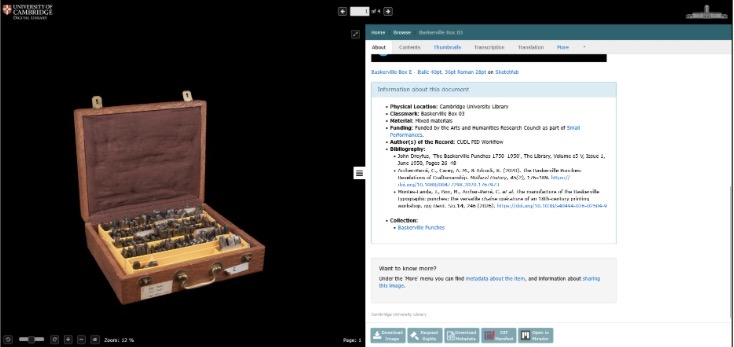
\includegraphics[width=0.8\textwidth]{./images/consultation_documents/IMG_5987.jpeg} 
	\caption{Mode de consultation proposant deux visionneuses}
	\label{fig:capture_ecran_deux_visionneuses}
\end{figure}

Une attention doit porter par la Bibliothèque Cujas face à ce choix, peu courant, car pensant s'adapter au mieux aux attentes des usagers, il ne faudrait pas que cela les rendent confus face à la présence de deux visionneuses. En effet, il semble que cela ne soit pas une habitude perpétrée par les institutions patrimoniales françaises car celle-ci propose uniquement une visionneuse \ac{IIIF}. Certains ont choisi la visionneuse Universal Viewer tandis que d'autres utilisent Mirador, répondant ainsi à des objectifs différents et des attentes propres à leurs usagers.

\subsection{L'interopérabilité des données et la pérennité des identifiants (ARK)}
Pour s'intégrer au web sémantique et aux grands réservoirs nationaux, comme le projet Orion de l'\ac{ABES}, le prototype s'appuie exclusivement sur des standards ouverts. La bibliothèque doit proposer des services permettant l'utilisation brute de données ainsi que des services d'export s'intégrant naturellement dans les chaînes de travail personnelles des chercheurs. Cette appropriation de la donnée par les chercheurs se heurte aujourd'hui à la volatilité des sessions de recherche \footannexe{\nameref{annexe_A_rapport_audit}.}.La concrétisation technique de ce "carnet de lecture" — dont nous avons justifié la nécessité méthodologique au chapitre précédent au prisme des travaux d'Elina Leblanc — pose directement la question de l'architecture de gestion des sessions dans le prototype. Afin de permettre aux chercheurs de sauvegarder leurs requêtes et leurs paniers de documents sans imposer une procédure d'inscription lourde, le prototype doit articuler deux options techniques : une persistance locale des données (via le local storage du navigateur de l'utilisateur, respectueuse de la vie privée) ou un système d'authentification fédérée (de type Shibboleth/Renater). Cette seconde piste s'avère la plus robuste pour assurer la pérennité des données de recherche d'une session à l'autre et sur différents terminaux \footcite{leblancBibliothequesNumeriquesEnrichies}. 

Afin de soutenir techniquement ces besoins d'appropriation et d'éditorialisation, l'architecture du prototype intègre des dispositifs d'interopérabilité spécifiques. Plutôt que de figer les données dans un silo de fichiers statiques, le prototype implémente des briques applicatives capables de concrétiser le concept de \enquote{citation de contenus} théorisé par Antoine Isaac, Emmanuelle Bermès et Gautier Poupeau \footcite{bermesWebSemantiqueBibliotheque2013}. En pratique, cette ambition se traduit par la mise en œuvre de modules spécifiques au sein du back-office (comme CopyIdRef ou Bibliography) et par l'exposition des métadonnées sous des formats de sérialisation ouverts (\ac{XML}, \ac{JSON-LD}). En associant à chaque document une \ac{URI} pérenne et un serveur d'images \ac{IIIF}, l'infrastructure technique ne se contente plus de diffuser : elle jette les bases d'un espace dynamique de co-construction de nouveaux savoirs, directement connectable aux outils personnels des chercheurs. Dans ce troisième âge, ce traitement intellectuel est l'un des moyens utilisés par les institutions patrimoniales transformant le document-objet en un espace d'apprentissage  et de valorisation du travail scientifique réalisés par des spécialistes.

Comme nous l'avons mis en évidence lors de l'étude comparative des outils de l'ESR, l'alternative représentée par Omeka S comporte d'importantes exigences en matière de maintenance applicative. Pour la \ac{BIU Cujas}, l'enjeu ne réside donc pas dans l'adoption passive d'un système clé en main, mais bien dans la maîtrise souveraine de ses flux de travail. En faisant le choix de développer le prototype sous Python-Django, l'institution privilégie une infrastructure sur-mesure et éco-conçue, capable de s'adapter précisément aux spécificités des sources juridiques tout en limitant la dépendance à des modules tiers dont la mise à jour n'est pas garantie à long terme.

Le choix de s'appuyer sur des formats universels et des \ac{API} vise à garantir la visibilité, la réutilisation et de la diffusion des collections à l'échelle nationale. Contrairement à l'entrepôt \ac{OAI-PMH} de CujasNum, devenu difficile à moissonner voir impossible, le prototype permet de réactiver le moissonnage en le standardisant davantage. Le système intègre dorénavant des \ac{API REST} capables de délivrer des données structurées et interopérables sous formats \ac{XML} ou \ac{JSON}, rompant avec l'image en silo \footnote{\nameref{annexe_A_rapport_audit}.}. Cette architecture modulaire offre une double opportunité : elle permet à la \ac{BIU Cujas} de moissonner d'autres portails comblant ces collections physiques ainsi que d'exposer ses propres métadonnées pour être moissonnées, augmentant drastiquement la visibilité de ses fonds.

Une des fortes attentes des chercheurs repose sur la stabilité à long terme des citations et de l'accès aux ressources numériques, pour qui la fiabilité d'un lien hypertexte est une condition importante de la scientificité de leurs travaux. À cette fin, il envisage \enquote{de désigner \ac{ARK} vers la notice bibliographique plutôt que le \ac{PDF}}. A la Bibliothèque Cujas, la méthode de création des identifiants pérennes est forgé à partir \enquote{du code-barre de l'ouvrage}, garantissant le lien permanent évitant les doublons. Cela permettrait ainsi de lier numériquement la notice bibliographique à celle du catalogue \footannexe{\nameref{annexe_A_rapport_audit}.}.

\subsection{La gestion fine des droits d'accès}
La bibliothèque numérique souhaite numériser des documents sous droit à intégrer dans sa nouvelle plateforme. Tout en restant dans un cadre strictement légal, la bibliothèque se doit de réfléchir à l'accès qu'elle permet à ses documents ne pouvant être exposés librement sans contrainte. Il est nécessaire pour l'établissement d'établir clairement une charte légale indiquant distinctement ce que l'usager a le droit de faire ou non concernant un document libre de droit et celui sous droit. La première étape consiste à assortir la notice du document à une \enquote{licence Etalab et/ou Creative Commons}. Cujas aimerait développer \enquote{un flitrage des documents sous droit ou libre de droit, grâce à la balise DcRight des notices Dublin Core} \footannexe{\nameref{annexe_A_rapport_audit}.}. 

\begin{figure}[htbp]
	\centering
	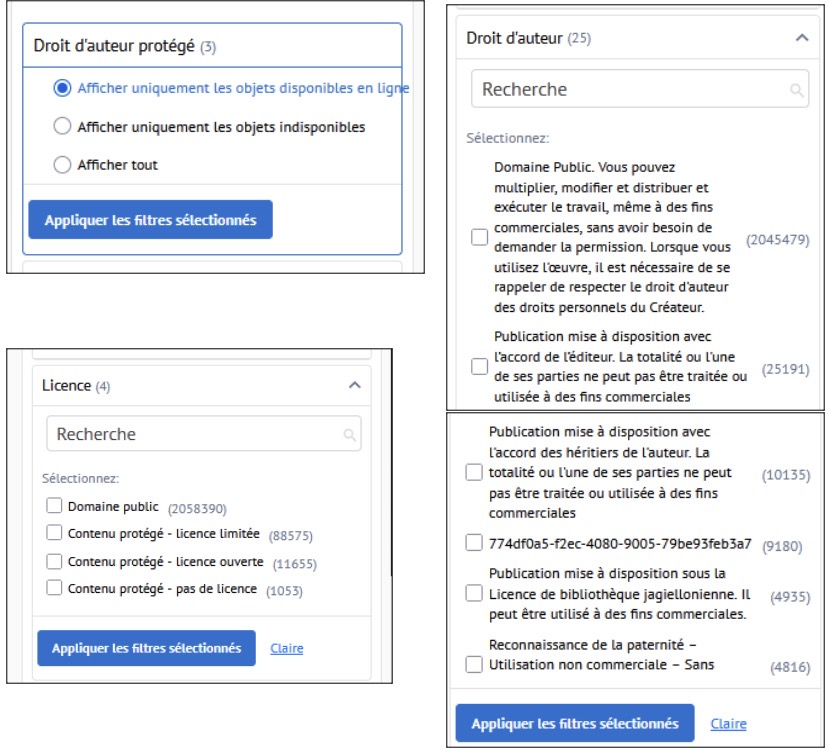
\includegraphics[width=0.5\textwidth]{./images/filtrage/IMG_5970.jpeg} 
	\caption{Différents types de filtrage dans Polona}
	\label{fig:capture_ecran_filtrage_Polona}
\end{figure}

Une des bibliothèques le fait également. Il s'agit de Polona, la bibliothèque nationale de Pologne, permettant de filtrer les documents sous droit. La deuxième étape serait de mettre en place \enquote{un horodatage débloquant le document sur le web une fois que les droits sont arrivés à terme}.

Le prototype permet de mettre en place des protocoles d'authentification centralisée \ac{SSO} et \ac{SAML}. En s'appuyant sur la fédération d'identité de Renater, grâce à ces protocoles, le système interroge à distance les serveurs des universités partenaires comme Paris I et Paris II. Cette architecture modulaire permet d'appliquer une gestion différenciée des droits d'accès \footannexe{ \nameref{annexe_A_rapport_audit}.}. Les métadonnées descriptives restent accessible publiquement sur le Web, tandis que la consultation des images est restreinte aux droits accordés par la bibliothèque en fonction du statut occupé par la personne. Un autre moyen d'accès, plus traditionnel, est de se connecter aux postes physiques connectés au réseau intranet local au sein de Cujas.

Sous \ac{XTF}, la chaîne de travail fonctionnait de façon chronophage. A l'origine, les experts métiers travaillaient de manière étanche, et toute modification de l'interface publique, une correction de coquille ou une mise en valeur éditoriale nécessitait l'intervention manuelle du service informatique. Le système était perçu comme une \enquote{boîte noire technique} par les experts métiers. Pour décloisonner ces processus, le prototype introduit un \enquote{back-office collaboratif structuré autour de profils et de rôles spécifiques}\footannexe{\nameref{annexe_A_rapport_audit} .}. 

Sur le plan de l'administration sémantique, Thomas Chaineux souligne qu'un tel environnement \enquote{répond à ses objectifs d’accès simplifié} et permet de \enquote{s’affranchir de la moindre écriture en format \ac{XML}/\ac{RDF}, \ac{JSON-LD} ou autre Turtle, grâce à l’ergonomie de son interface}. Pour la mise en valeur et l'éditorialisation, \enquote{la création de ces pages est simplifiée, de sorte qu’aucune compétence en modélisation de page Web (\ac{HTML} ou CSS) n’est requise}, l'écriture s'effectuant via une interface d'édition visuelle intuitive \footcite{chaineuxLentreeDansWeb}.

Cette autonomie s'accompagne d'une sécurisation des données grâce à la mise en œuvre de resource templates, définis par Thomas Chaineux comme \enquote{des formulaires [...] permettant de s’assurer que toutes les entités seront décrites de la même manière}, ce qui facilite la transmission et garantit la pérennité des schémas documentaires au fil du temps. Enfin, à l'image des rôles d'administration d'un \ac{CMS} sémantique, le système \enquote{propose des solutions différentes selon le statut de l’utilisateur}, permettant par exemple à un chercheur d'éditorialiser un fonds spécifique de manière autonome, tout en réservant l'accès à la base de données globale aux seuls administrateurs techniques \footcite{chaineuxLentreeDansWeb}. Cette gestion des rôles permettrait à la Bibliothèque Cujas, par exemple, \enquote{à un agent ou à un chercheur de rédiger et publier un texte sur le fonds qu'il a traité, sans pour autant lui donner les droits d'administrateur global sur tout le système}\footannexe{\nameref{annexe_A_rapport_audit}.}.    

\section[Dilemme de l'infrastructure]{Le dilemme de l'infrastructure: entre le sur-mesure et le standard}
La refonte de la bibliothèque numérique de la \ac{BIU Cujas} soulève une interrogation stratégique dépassant la simple technique informatique : quel modèle d'infrastructure privilégier pour garantir à la fois l'indépendance et l'adéquation aux besoins scientifiques et la pérennité de l'outil ? En ingénierie documentaire, c'est une question classique opposant la logique du développement spécifique, incarné par le prototype Codex, à celle de l'adoption d'outil standard, comme Omeka S.

\subsection{L'analyse du sur-mesure}
Le choix initial de la Bibliothèque Cujas, en développant le prototype Codex, offre une flexibilité totale et une forte adaptation aux besoins métiers. Cela évite également la dépendance finiancière et technique vis-à-vis d'un prestataire externe, \enquote{qui facture cher la moindre évolution}. Conçu en Python-Django, Codex offre l'avantage de s'interfacer dans la façon de travailler des experts métiers. Ce couplage permettrait  d'automatiser certaines tâches de la chaîne de numérisation de Cujas, comme la génération de métadonnées \ac{METS} ou \ac{XML}, ou des transferts sécurisés vers le serveur d'archivage du \ac{CINES}.

Si l'adaptation aux besoins est forte, ce mode de développement démontre une extrême vulnérabilité humaine, identifiée, par le directeur de la bibliothèque. Il le perçoit comme un risque de pérennité de l'infrastructure en bâtissant la future bibliothèque numérique uniquement sur les compétences d'une seule personne. En effet, Olesea Dubois confirme cette analyse : \enquote{le plus gros soucis avec les outils maisons c'est qu'ils sont très souvent associés à des personnes et à des procédures qui leur sont propres}\footannexe{\nameref{annexe_A_rapport_audit}}[pour voir l'entretien réalisé auprès d'Olesea Dubois]. Un autre inconvénient mis en avant par la responsable de la bibliothèque numérique de Sciences Po est que \enquote{généralement, il y a peu ou pas assez de documentations entraînant ainsi une durée de vie assez courte de la bibliothèque numérique} \footannexe{\nameref{annexe_A_rapport_audit} pour voir l'entretien avec Olesea Dubois.}. Effectivement, le peu de documentation disponible entraîne un risque pour la pérennité de l'outil, et empêche le maintien sur le long terme de la bibliothèque numérique. Avoir recours à un logiciel sur-mesure entraîne une difficulté de recrutement, car l'institution se coupe d'un vivier de compétence, rendant rapidement le code sur-mesure inexploitable en cas du départ de son concepteur, condamnant le système à une obsolescence rapide. La crainte de la plupart des institutions patrimoniales y compris la bibliothèque Cujas est de reproduire la situation qui a entraîné la disparition de la bibliothèque numérique Medica. C'est pour pallier à cela qu'elles ont choisi de se tourner vers des outils standardisés afin de disposer d'un vivier de personnel.

La tension entre le développement d’un prototype sur-mesure et l’adoption d’un standard communautaire comme Omeka S s'inscrit au cœur des réflexions sur la souveraineté technique et la maîtrise de l'obsolescence logicielle au sein des institutions patrimoniales\footcite{bermesWebSemantiqueBibliotheque2013}. D'un côté, le développement interne d’une solution ad hoc, à l'instar du prototype \textit{Codex} conçu sous Python-Django, s'impose comme une réponse souveraine et immédiate face à l'urgence fonctionnelle : il permet de pallier la fragilité de CujasNum sous l'infrastructure obsolète \ac{XTF} et d'assurer une continuité absolue du service public de la recherche face aux risques de sécurité informatique. 

Toutefois, cette autonomie technique se heurte rapidement aux limites de la maintenance à long terme d'un outil isolé. À l'ère de la Transition bibliographique, la rapidité des évolutions technologiques rend en effet indispensable l'adossement à une communauté active pour éviter qu'une institution ne se retrouve marginalisée par des services rapidement dépassés. C'est ici que l'adoption d'un standard libre et communautaire tel qu'Omeka S révèle sa force stratégique. En s'appuyant sur un code source ouvert, l'établissement lutte activement contre l'obsolescence logicielle souvent entretenue par les éditeurs de logiciels propriétaires\footcite{creusotQuellesPerspectivesPour}. De plus, en permettant un déploiement et un hébergement locaux — contrairement aux offres propriétaires en mode SaaS (\textit{Software as a Service}) sur le cloud —, un outil comme Omeka S garantit à l’institution la maîtrise absolue de ses données et de ses choix d'archivage, réalisant un compromis idéal entre les impératifs du modèle sémantique sémantisé (RDF, Dublin Core) et l'utilisabilité de l'interface\footcite{chaineuxLentreeDansWeb, creusotQuellesPerspectivesPour}.


\subsection{L'analyse du standard communautaire}
Face au risque d'isolement technique du sur-mesure, les retours d'expérience des responsables de bibliothèque numérique des institutions patrimoniales comme la Bibliothèque Sainte-Geneviève, la Bibliothèque de Sciences Po ou l'\ac{ENS}, démontrent un abandon progressif des outils sur-mesure au profit d'Omeka S. Financé par des subventions de recherche, de fondations et soutenu par une communauté, Omeka S offre des garanties majeures de durabilité. Comme le résume Thomas Chaineux, ce logiciel représente \enquote{un compromis entre les impératifs du modèle et l'ergonomie}, s'imposant pour les \ac{BU} moyennes comme \enquote{une porte d'entrée bienvenue} grâce à sa gratuité et la force de son réseau communautaire \footcite{chaineuxLentreeDansWeb}. Contrairement à Django qui nécessite d'avoir des compétences informatiques avancées pour développer le logiciel et l'intégrer dans le web sémantique. La particularité d'Omeka S est d'avoir été pensé pour s'intégrer directerement ou plus facilement dans le web de données. Il s'appuie sur une \enquote{modélisation des métadonnées sous \ac{RDF}} combinées à des vocabulaires standardisés, comme le Dublin Core, qui favorise \enquote{une meilleure exposition des données}. Il facilite l'exposition des métadonnées, leur exportation et leur interopérabilité. 
 
De plus, un autre des avantages pour les catalogueurs est de \enquote{bénéficier d'un back-office documenté, collaboratif et modulaire}. Toutefois, malgré les avantages certains, l'environnement Omeka S s'accompagne de contraintes réelles. Bien qu'open-source, le logiciel est \enquote{gratuit}, mais il exige des ressources pour fonctionner et évoluer. Omeka S demande des ressources internes pour en assurer l'hébergement, le paramétrage et la maintenance technique. Gilles Clément, l'un des concepteurs de NuBIS, témoigne de cette limite : \enquote{À l'usage, chaque nouvelle version d'Omeka S cassait quelque chose[...]. Nous étions confrontés à beaucoup de bidouillages en raison de l'instabilité des modules tiers développés par des prestataires différents, ce qui rendait le code lourd et difficile à maintenir} \footannexe{\nameref{annexe_A_rapport_audit} pour voir l'entretien avec Cécile Obligi et Gilles Clément de la \ac{BIS}.}. Cette instabilité fait écho à l'analyse de Thomas Chaineux, qui situe Omeka S dans \enquote{une position hybride dans le Web de données}. Faute d'émettre des \ac{URI} nativement pérennes à l'échelle globale sans développements tiers, le logiciel génère par défaut des \enquote{noeuds blancs} dont la portée reste limitée au contexte local \footcite{chaineuxLentreeDansWeb}. 
 
Face à cet obstacle, la solution mise en place par la \ac{BIS} pour le résoudre, a été de séparer techniquement le front du back, \enquote{rendant ainsi le code-source plus maintenable dans le temps} \footannexe{\nameref{annexe_A_rapport_audit} pour voir l'entretien avec Cécile Obligi et Gilles Clément de la \ac{BIS}.}. En effet, à chaque mise à jour, le module complémentaire déréglait les paramétrages du front-office. La \ac{BIS} a donc découplé son architecture en décidant de \enquote{développer leur back-office sous Omeka S et du front sous Astro.js} \footannexe{\nameref{annexe_A_rapport_audit} pour voir l'entretien avec Cécile Obligi et Gilles Clément de la \ac{BIS}.}. Cette distinction rend étanche les couches logicielles permettant ainsi le bon fonctionnement de NuBIS et la satisfaction des équipes qui en sont en charge. Malgré cet obstacle rencontré par certaines institutions, l'open-source, contrairement au sur-mesure, a cette \enquote{notion de mutualisation rendant plus facile l'idée du maintien de cette structure} \footannexe{\nameref{annexe_A_rapport_audit} pour voir l'entretien avec Vincent Tardif de l'\ac{ENS}.}. Le choix de la \ac{BIS} du framework Astro.js répond à des exigences d'éco-conception et d'accessibilité numérique, évitant ainsi l'interrogation de la base à chaque clic de l'usager. L'avantage majeur de ce type de fonctionnement est que les montées de versions d'Omeka S n'impactent plus l'affichage public, sécurisant mieux le back-office le rendant plus maintenable dans le temps et pérenne.
\section{Pérennité, maintenance et gestion des risques}
Le passage d'\ac{XTF} vers un nouveau système ne se limite pas uniquement à un arbitrage d'ingénierie logicielle. Il constitue un défi de gouvernance et de gestion des ressources humaines et de viabilité du logiciel sur le long terme pour la Bibliothèque Cujas.

Tout d'abord, à l'instar d'autres bibliothèques, l'ensemble de l'infrastructure technique repose principalement sur les compétences d'une seule personne. Ce constat d'une dépendance extrême est reconnu par le directeur et les experts métiers, attendant avec la nouvelle infrastructure d'avoir une meilleure visibilité dans le back-office. Pour éviter de créer à nouveau une \enquote{boîte noire} et d'abrégrer prématurément la durée de vie de la bibliothèque numérique, toute refonte doit alors s'accompagner d'une documentation fonctionnelle et technique très détaillée \footannexe{\nameref{annexe_A_rapport_audit}.}. Cette documentation permet ainsi de comprendre et de justifier les choix qui ont été fait. Elle doit consigner \enquote{chaque choix de circuit, l'architecture des bases de données, le code des \ac{API} et la configuration des serveurs} permettant ainsi de disposer d'une compréhension globale dans le cas du départ du concepteur, remplacé par une autre personne assurant sa pérennité \footannexe{ \nameref{annexe_A_rapport_audit}.}.
	
	\begin{figure}[htbp]
		\centering
		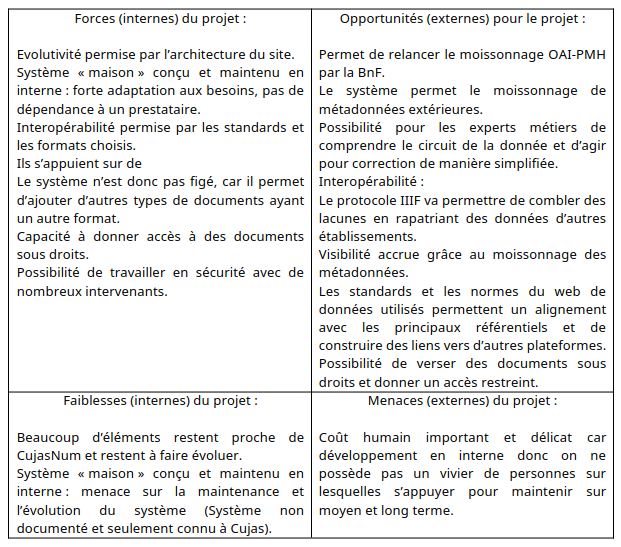
\includegraphics[width=0.5\textwidth]{./images/Screenshot from 2026-09-07 20-54-20.png} 
		\caption{Réalisation d'un SWOT pour le prototype}
		\label{fig:capture_ecran_SWOT}
	\end{figure}
	
	
Le choix de pérenniser un prototype sur-mesure amène la Bibliothèque Cujas à devoir assurer la totalité de \enquote{l'effort de maintenance corrective en interne, de mise à jour des sécurités et à l'adaptation à de futurs standards} \footannexe{\nameref{annexe_A_rapport_audit}.}. Or, la Bibliothèque Cujas ne dispose pas d'un vivier de développeurs permettant d'assurer un suivi de la bibliothèque numérique. À l'inverse de la maintenance d'un système open-source qui permet de partager l'effort, réduisant la charge technique.

La refonte de la bibliothèque numérique de la Bibliothèque cujas ne saurait se résumer uniquement à un simple chantier informatique. Les choix d'infrastructure posent les fondations matérielles et logicielles indispensables à la pérennité, à la sécurité et à l'interopérabilité des collections patrimoniales. Cependant, aussi évolué que peut être l'ingénierie logicielle, elle ne serait être validée si elle ne s'adapte pas aux pratiques contemporaines de la recherche. Il est donc nécessaire d'évaluer comment mettre en place des services fluides adaptés à l'usage.